%++++++++++++++++++++++++++++++++++++++++
% Don't modify this section unless you know what you're doing!
\documentclass[letterpaper,12pt]{article}
\usepackage{tabularx} % extra features for tabular environment
\usepackage{amsmath}  % improve math presentation
\usepackage{graphicx} % takes care of graphic including machinery
\usepackage[margin=1in,letterpaper]{geometry} % decreases margins
\usepackage{cite} % takes care of citations
\usepackage[final]{hyperref} % adds hyper links inside the generated pdf file
\hypersetup{
	colorlinks=true,       % false: boxed links; true: colored links
	linkcolor=blue,        % color of internal links
	citecolor=blue,        % color of links to bibliography
	filecolor=magenta,     % color of file links
	urlcolor=blue         
}
\usepackage{tikz}
%++++++++++++++++++++++++++++++++++++++++


\begin{document}

\title{Physical Education 77: Virtual Fitness}
\date{Location: The Big C || Time: 3-6 Fridays }
\author{Instructors: Emily Harari, Loren Curry, Rachel Elia, Melissa Constantino}
\maketitle

\section{General Information}
In this DeCal, we will work to improve physical fitness, endurance, and respiratory strength through fun and engaging workouts. Our daily warm up will be the walk to the top of the Big C, and from there we will engage in different workout programs such as Just Dance, Wii Sports, and other virtual fitness games and programs. Students will learn a variety of fitness techniques in class that they can apply to their everyday fitness schedule. By the end of this course, students will have a large knowledge of workouts to improve their own fitness, as is the goal of the Physical Education program at UC Berkeley.  

\section{Course Requirements and Policies}

All students must have a fun and positive attitude toward trying new things. There are no prior pre-requisites necessary to take this course. There is one required reading which will help to build on the information covered in the class. The material from the book will be included in the final physical test.\\
\\
Required Reading: The 4-Hour Body by Tim Ferriss \\
\\
Attendance is not mandatory. However, it is a very large portion of your grade and crucial to your success in this class. It is impossible to pass this class if you do not attend it on a regular basis. Lateness of 30+ minutes past Berkeley time will be considered as 1/2 of an absence.\\
\\
As you are all adults, we will allow you to make your own decisions about using technology in class. However, excessive use of technology in class will be factored into your grade for participation and enthusiasm. Plagiarism will not be tolerated. Any evidence of cheating will result in immediate failure
of the course as per university policy. You are required to maintain the academic honesty as per university guidelines. 

\section{Office Hours}
It is highly encouraged that students attend office hours. This time is crucial for students to ask questions on subjects they struggle with, expand their knowledge, and get to know the instructors. They are crucial for the success in this course. \\
Loren Curry: M,W 10-11 in Evans 333 \\
Emily Harari: T,TH 10-11 in Stanley 205\\
Rachel Elia: M 4-6 at Memorial Glade\\
Melissa Constantino: F 12-2 at Cafe Milano


\section{Grading}
Grades for this class will be determined as follows:
\begin{table}[ht]
\begin{center}
\caption{Grade Distribution}
\label{tbl:bins} % spaces are big no-no withing labels
\begin{tabular}{|cc|} 
\hline
\multicolumn{1}{|c}{Assignments} & \multicolumn{1}{c|}{Weight} \\
\hline
Attendance &   30\% : 45 points \\
Workout Project &   20\% : 30 points \\
Participation and Enthusiasm &   20\%: 30 points \\
Physical Test &  20\% : 30 points \\
\hline
\end{tabular}
\end{center}
\end{table}

This class is 2 units, P/NP only. 105+/150 points is required to pass the course.   Attendance is worth 30\%\ of the overall grade. There will be one project worth 30 points. Participation and visible enthusiasm is worth 30 points. A physical test at the end of the semester is worth 30 points.

All grades will be uploaded to bcourses, so that students may know their progress in the class. Additional surveys will be sent out during the semester to gain feedback from students on the course.


\section{Calendar}
\begin{table}[ht]
\begin{center}
\caption{Course Schedule}
\label{tbl:bins} % spaces are big no-no withing labels
\begin{tabular}{|cc|} 
\hline
\multicolumn{1}{|c}{DATE} & \multicolumn{1}{c|}{TOPIC} \\
\hline
8/31/18 &   Introduction -- Squats and Push-Ups \\
9/7/18 &   Just Dance 3on the Wii \\
9/14/18 &   Wii Fit -- Tennis \\
9/21/18 &   Wii Fit -- Yoga \\
9/28/18 &   Wii Fit -- Pilates pt. 1\\
10/5/18 &   Wii Fit -- Pilates pt. 2\\
10/12/18 &  Just Dance 4 on the Wii\\
10/19/18 &  Wii Fit -- Aerobics, Jump Roping \\
10/26/18 &  Wii Fit -- Aerobics, Jogging \\
11/2/18 &   Wii Fit -- Aerobics, Hula Hooping \\
11/9/18 &   Ab Workout \\
11/16/18 &  Final Project Due; Review of squats, push-ups, and abs \\
11/23/18 &  Thanksgiving Break -- No Class \\
11/30/18 &  Physical Fitness Test \\
\hline
\end{tabular}
\end{center}
\end{table}

The Final Project rubric will be handed out the 4th week of classes. In the project, you will be expected to create your own workout routine and present it to one of the instructors.\\
\\
For the physical fitness test, you will be tested on your knowledge of three of the following: Wii Fit Tennis, Yoga, Pilates, Jump Roping, Jogging, and Hula Hooping. As well as one of the following: squats, push ups, or abs. \\
\\
Below is a Course Schedule and Venn Diagram of the overall goals and topics of this class. 

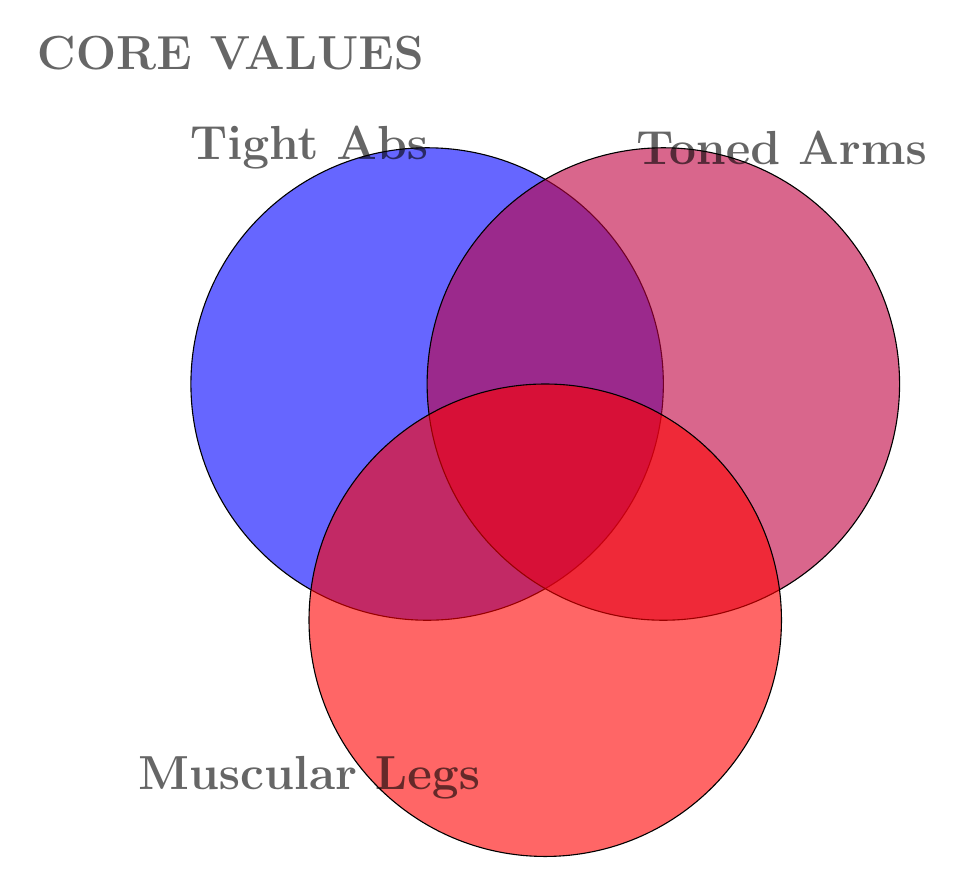
\begin{tikzpicture}
	\begin{scope} [fill opacity = .6]
    \draw[fill=blue, draw = black] (-1.5,1) circle (3);
    \draw[fill=purple, draw = black] (1.5,1) circle (3);
    \draw[fill=red, draw = black] (0,-2) circle (3);
    \node at (-4,5.2) {\LARGE\textbf{CORE VALUES}};
    \node at (-3,4) {\LARGE\textbf{Tight Abs}};
    \node at (3,4) {\LARGE\textbf{Toned Arms}};
    \node at (-3,-4) {\LARGE\textbf{Muscular Legs}};
    \end{scope}
\end{tikzpicture}


\end{document}



